\chapter{Конструкторская часть}

В данном разделе представлены схемы алгоритмов умножения матриц и произведена оценка трудоемкости алгоритмов умножения матриц.

\section{Разработка стандартного алгоритма умножения матриц}
На рисунке \ref{img:standard_alg} представлена схема стандартного алгоритма умножения матриц.

\begin{figure}[h!]
\centering
    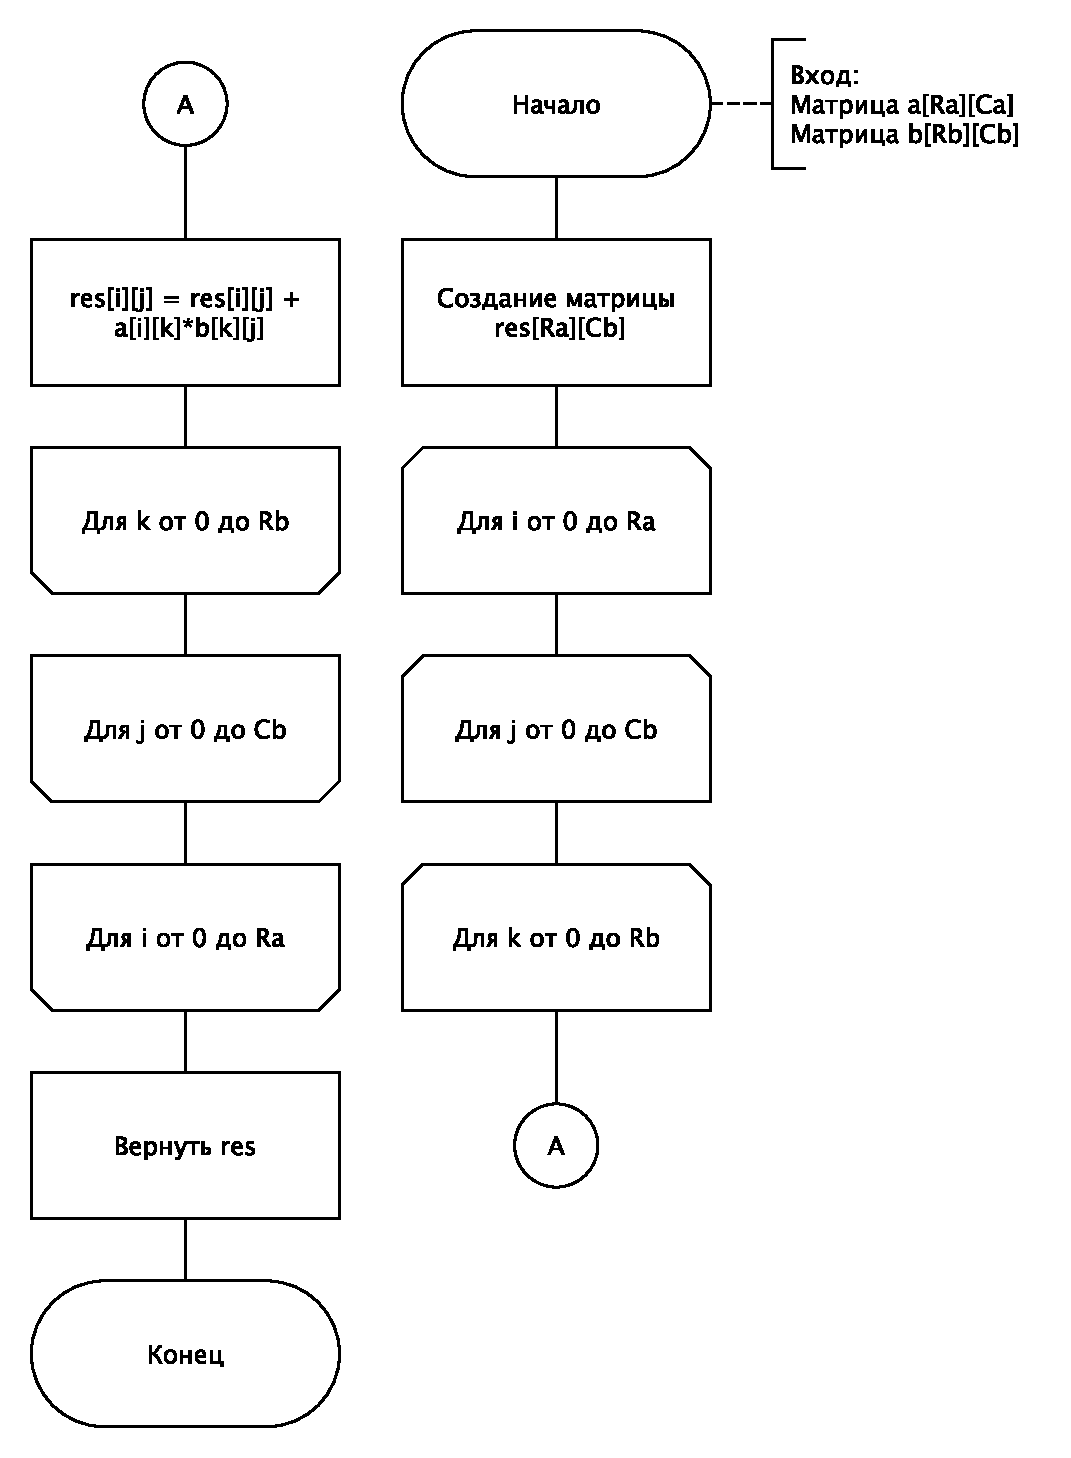
\includegraphics[width=0.6\linewidth]{standard.pdf}
    \caption{Схема стандартного алгоритма умножения матриц}
    \label{img:standard_alg}	
\end{figure}

\newpage

\section{Разработка алгоритма Винограда}
На рисунках \ref{img:winograd_alg}~--~\ref{img:winograd_func_alg} представлена схема алгоритма Винограда для умножения матриц. 

\begin{figure}[h!]
    \centering
    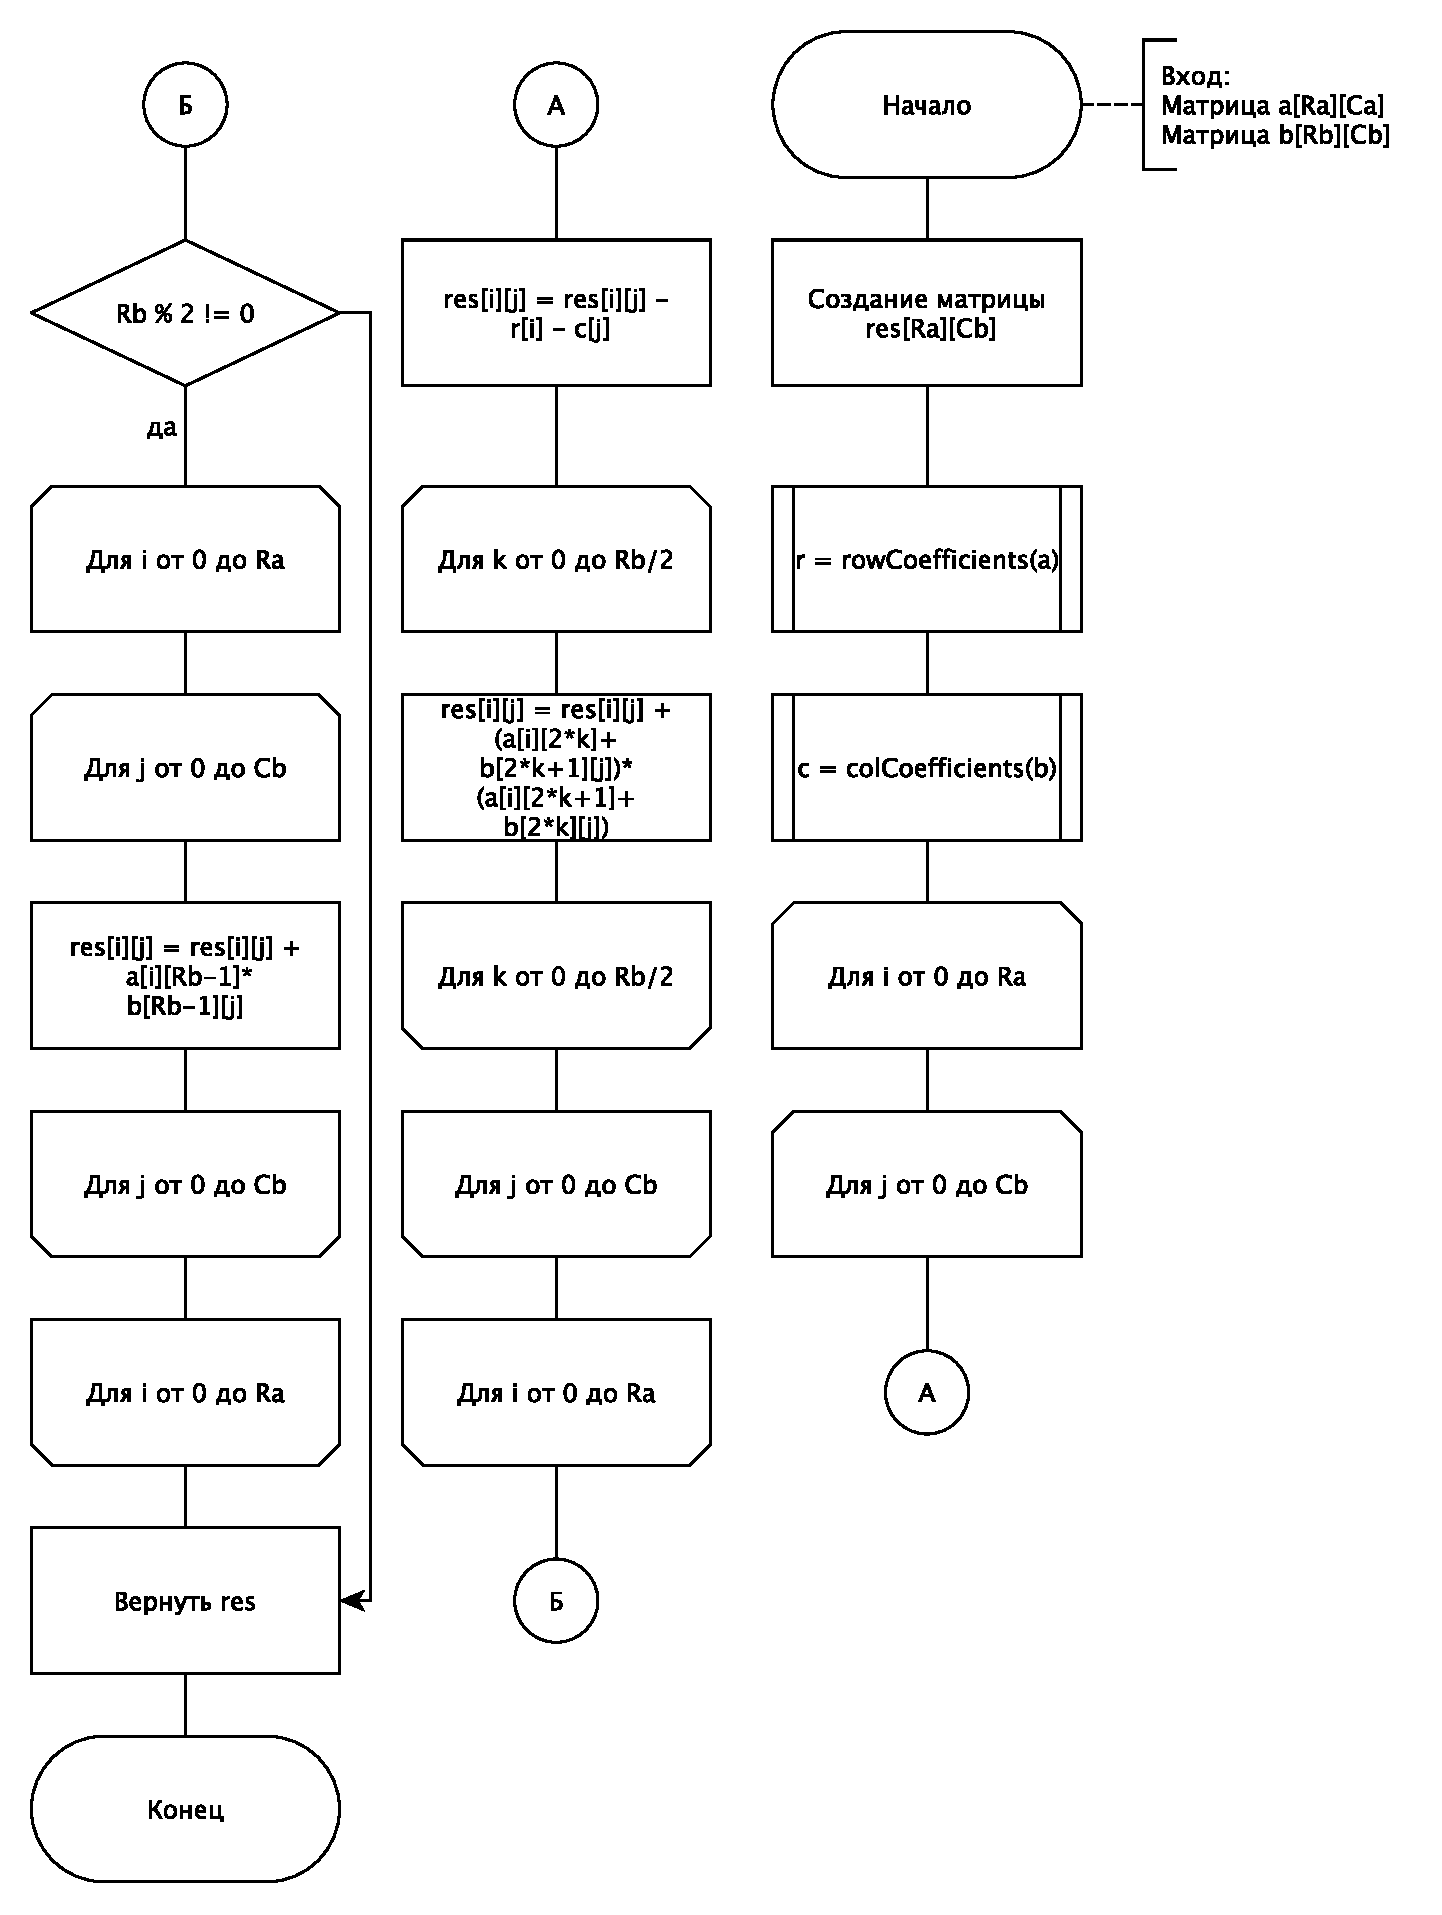
\includegraphics[width=0.9\linewidth]{winograd.pdf}
    \caption{Схема алгоритма Винограда для умножения матриц}
    \label{img:winograd_alg}
\end{figure}

\newpage

\begin{figure}[h!]
    \centering
    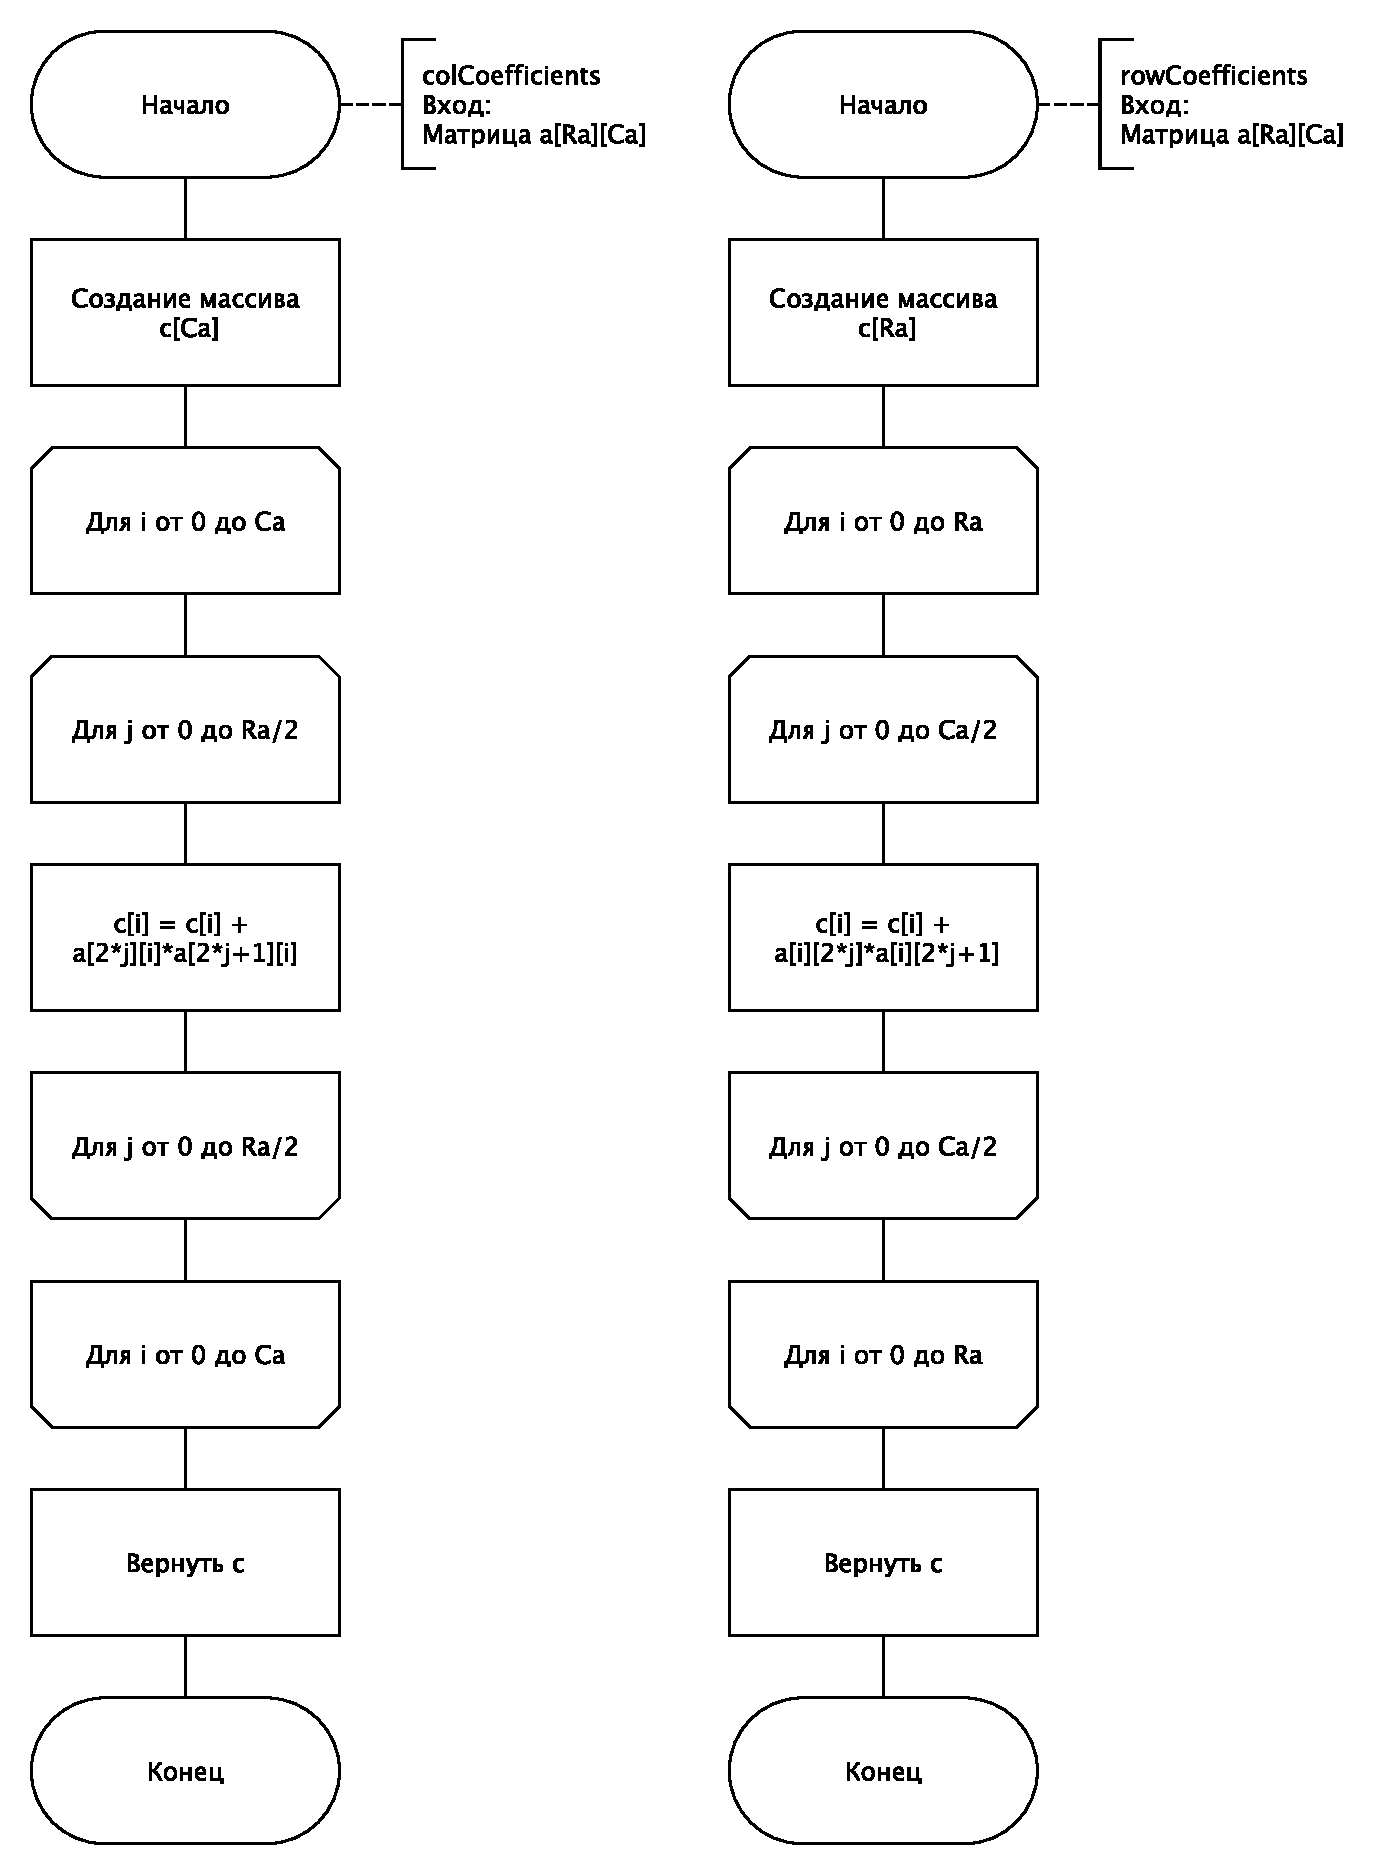
\includegraphics[width=0.9\linewidth]{winograd_func.pdf}
    \caption{Схема алгоритма Винограда для умножения матриц (функции нахождения произведений соседних элементов строк и столбцов)}
    \label{img:winograd_func_alg}
\end{figure}

\newpage

\section{Разработка оптимизированного алгоритма Винограда}
На рисунках \ref{img:winograd_improved_alg}~--~\ref{img:winograd_improved_func_alg} представлена схема оптимизированного алгоритма Винограда.

\begin{figure}[h!]
    \centering
    \includegraphics[width=1\linewidth]{winograd_improved}
    \caption{Схема оптимизированного алгоритма Винограда}
    \label{img:winograd_improved_alg}
\end{figure}

\newpage

\begin{figure}[h!]
    \centering
    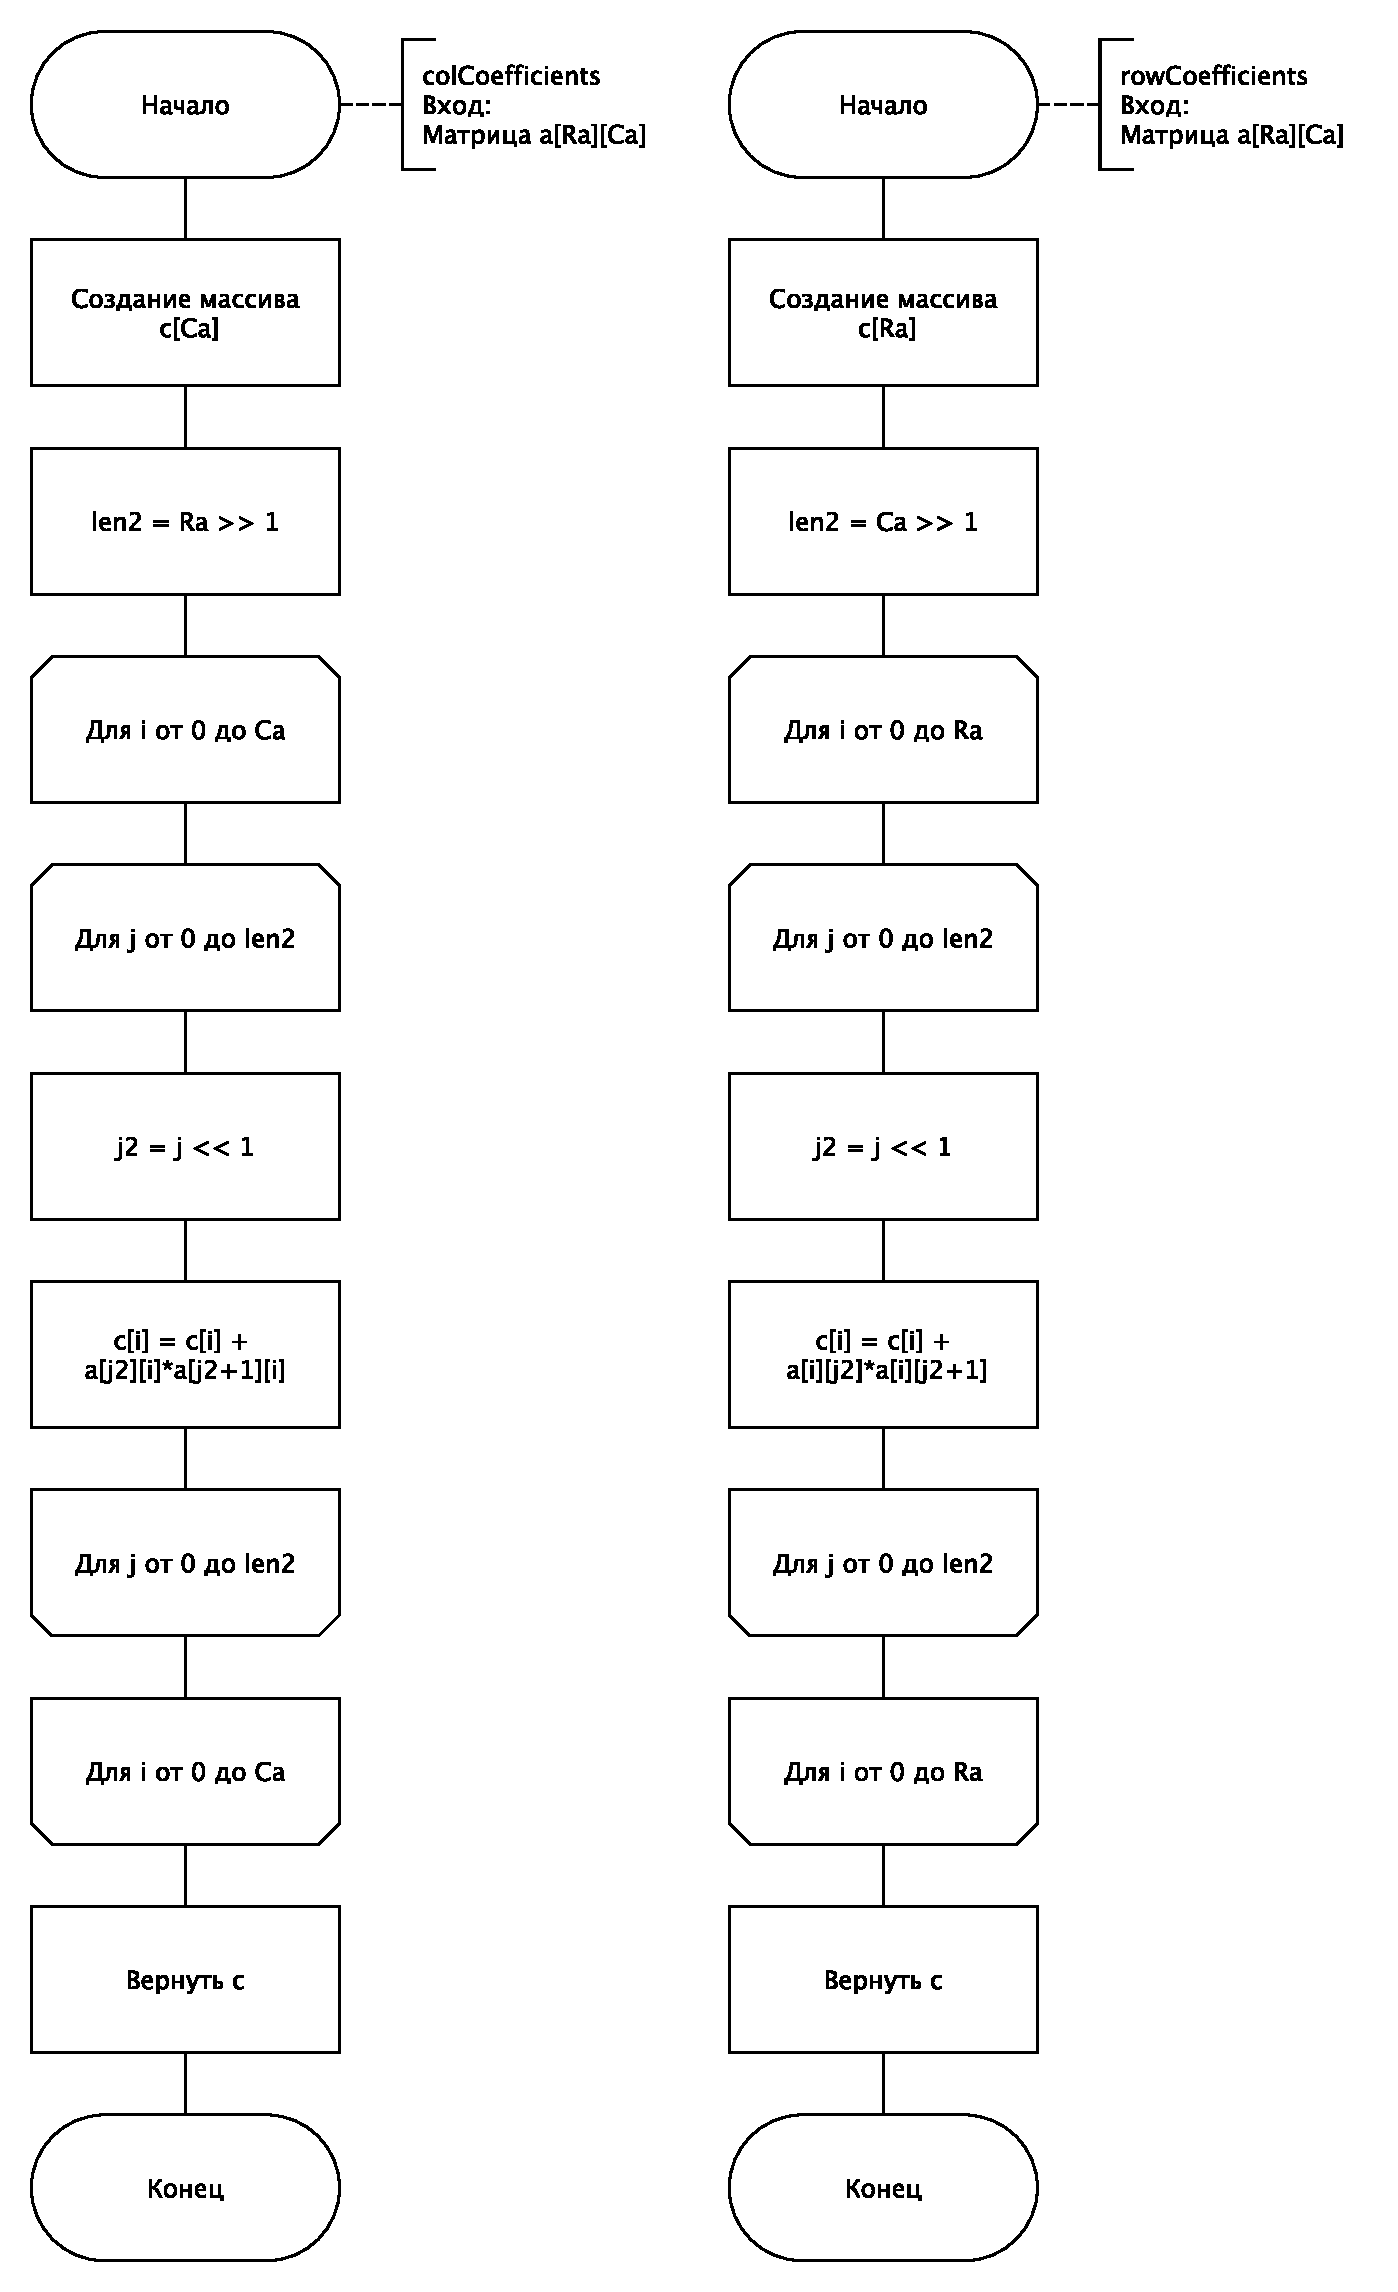
\includegraphics[width=0.75\linewidth]{winograd_improved_func.pdf}
    \caption{Схема алгоритма Винограда для умножения матриц (функции нахождения произведений соседних элементов строк и столбцов)}
    \label{img:winograd_improved_func_alg}
\end{figure}

\newpage

\section{Оценка трудоемкости алгоритмов умножения матриц}

\subsection{Модель вычислений}
Для вычисления трудоемкости исследуемых алгоритмов необходимо ввести модель вычислений. 

Если обозначить трудоемкость некоторой операции $a$, как $f_a$, то можно ввести таблицу соответствия значения трудоемкости для базовых операций:


\begin{table}[h]
  \caption{\label{table:complexity} Таблица значений тредоемкости}
  \begin{center}
    \begin{tabular}{|l|r|}
      \hline
      Операция & Трудоемкость\\ \hline
      $:=$ & $1$ \\ \hline
      $+=$ & $1$ \\ \hline
      $-=$ & $1$ \\ \hline
      $+$ & $1$ \\ \hline
      $-$ & $1$ \\ \hline
      $<<$ & $1$ \\ \hline
      $>>$ & $1$ \\ \hline
      $[]$ & $1$ \\ \hline
      $++$ & $1$ \\ \hline
      $--$ & $1$ \\ \hline
      $>=$ & $1$ \\ \hline
      $<=$ & $1$ \\ \hline
      $==$ & $1$ \\ \hline
      $!=$ & $1$ \\ \hline
      $<$ & $1$ \\ \hline
      $>$ & $1$ \\ \hline
      $*$ & $2$ \\ \hline
      $/$ & $2$ \\ \hline
      $\%$ & $2$ \\ \hline
      вызов функции & $0$ \\ \hline
    \end{tabular}
  \end{center}
\end{table}

Трудоемкость условного блока можно ввести следующим образом:

\begin{equation}
	f_{if} = f_{cond} + \begin{cases}
		min(f_{in\_if}, f_{in\_else}) \quad \text{в лучшем случае}, \\
		max(f_{in\_if}, f_{in\_else}) \quad \text{в худшем случае},
	\end{cases}
\end{equation}

где

\begin{itemize}
	\item $f_{if}$~---~трудоемкость условного блока;
	\item $f_{cond}$~---~трудоемкость вычисления условия;
	\item $f_{in\_if}$~---~трудоемкость фрагмента после $if$;
	\item $f_{in\_else}$~---~трудоемкость фрагмента после $else$.
\end{itemize}

Трудоемкость цикла можно ввести следующим образом:


\begin{equation}
	f_{loop} = f_{init} + f_{cmp} + n \cdot (f_{body} + f_{cmp} + f_{inc}),
\end{equation}

где

\begin{itemize}
	\item $f_{loop}$~---~трудоемкость цикла;
	\item $f_{init}$~---~трудоемкость инициализирующего выражения;
	\item $f_{cmp}$~---~трудоемкость сравнения цикла;
	\item $f_{body}$~---~трудоемкость тела цикла;
	\item $f_{inc}$~---~трудоемкость инкремента.
\end{itemize}

\subsection{Трудоемкость стандартного алгоритма умножения матриц}
Здесь и далее будут использоваться следующие обозначения:

\begin{itemize}
	\item $N$~---~количество строк первой матрицы;
	\item $M$~---~количество столбцов первой матрицы (количество строк второй матрицы);
	\item $K$~---~количество столбцов второй матрицы. 
\end{itemize}

Трудоемкость внутреннего цикла по $k$ равна

\begin{equation}
	f_1 = 2 + M \cdot (2 + 12) = 2 + M \cdot 14.
\end{equation}

Трудоемкость внутреннего цикла по $j$ равна

\begin{equation}
	f_2 = 2 + K \cdot (2 + f_1).
\end{equation}

Трудоемкость алгоритма равна трудоемкости внешнего цикла по $i$

\begin{equation}
	f = 2 + N \cdot (2 + f_2) = 2 + N \cdot (2 + 2 + K \cdot (2 + f_1)),
\end{equation}

\begin{equation}
	f = 2 + N \cdot (2 + 2 + K \cdot (2 + 2 + M \cdot 14)),
\end{equation}

\begin{equation}
	f = 2 + N \cdot 4 + N \cdot K \cdot 4 + N \cdot K \cdot M \cdot 14 \approx 14 \cdot N \cdot M \cdot K.
\end{equation}

\subsection{Трудоемкость алгоритма Винограда}

Для алгоритма Винограда худшим случаем будет ситуация, в которой количество строк во второй матрице нечетное. Если оно четное, то это лучший случай.

Трудоемкость создания массива сумм произведений соседних элементов строк равна

\begin{equation}
	f_1 = 2 + N \cdot (2 + 2 + \frac{M}{2} \cdot 19) = 2 + N \cdot 4 + N \cdot M \cdot 9.5.
\end{equation}

Трудоемкость создания массива сумм произведений соседних элементов столбцов равна

\begin{equation}
	f_2 = 2 + K \cdot (2 + 2 + \frac{M}{2} \cdot 19) = 2 + K \cdot 4 + K \cdot M \cdot 9.5.
\end{equation}

Трудоемкость внутреннего цикла по $k$ равна

\begin{equation}
	f_3 = 2 + \frac{M}{2} \cdot (2 + 26) = 2 + M \cdot 14.
\end{equation}

Трудоемкость внутреннего цикла по $j$ равна

\begin{equation}
	f_4 = 2 + K \cdot (2 + f_3 + 8) = 2 + K \cdot 12 + K \cdot M \cdot 14.
\end{equation}

Трудоемкость внешнего цикла по $i$ равна

\begin{equation}
	f_5 = 2 + N \cdot (2 + f_4) = 2 + N \cdot 2 + N \cdot K \cdot 12 + N \cdot K \cdot M \cdot 14.
\end{equation}

Трудоемкость условия после основных циклов равна

\begin{equation}
	f_6 = 3 + \begin{cases}
		0, & \text{лучший случай}, \\
		2 + N \cdot 2 + N \cdot K \cdot 13, & \text{худший случай}.
	\end{cases}
\end{equation}

Тогда, трудоемкость алгоритма Винограда равна

\begin{equation}
	f = f_1 + f_2 + f_5 + f_6,
\end{equation}

\begin{equation}
	f \approx \begin{cases}
		N \cdot K \cdot M \cdot 14, & \text{лучший случай}, \\
		N \cdot K \cdot M \cdot 14, & \text{худший случай}.
	\end{cases}
\end{equation}

\subsection{Трудоемкость оптимизированного алгоритма Винограда}

Трудоемкость создания массива сумм произведений соседних элементов строк равна

\begin{equation}
	f_1 = 2 + N \cdot (2 + 2 + \frac{M}{2} \cdot 12) = 2 + N \cdot 4 + N \cdot M \cdot 6.
\end{equation}

Трудоемкость создания массива сумм произведений соседних элементов столбцов равна

\begin{equation}
	f_2 = 2 + K \cdot (2 + 2 + \frac{M}{2} \cdot 12) = 2 + K \cdot 4 + K \cdot M \cdot 6.
\end{equation}

Трудоемкость внутреннего цикла по $k$ равна

\begin{equation}
	f_3 = \begin{cases}
		4 + M \cdot 8.5, \quad \text{лучший случай}, \\
		4 + M \cdot 14, \quad \text{худший случай}.
	\end{cases}
\end{equation}

Трудоемкость внутреннего цикла по $j$ равна

\begin{equation}
	f_4 = 2 + K \cdot 8 + K \cdot f_3) = \begin{cases}
 	2 + K \cdot 12 + K \cdot M \cdot 8.5, \quad \text{лучший случай}, \\
 	2 + K \cdot 12 + K \cdot M \cdot 14, \quad \text{худший случай}.
 \end{cases}

\end{equation}

Трудоемкость внешнего цикла по $i$ равна

\begin{equation}
	f_5 = 2 + N \cdot 2 + N \cdot f_4 = \begin{cases}
 	2 + N \cdot 4 + N \cdot K \cdot 12 + N \cdot K \cdot M \cdot 8.5, \quad \text{лучший случай}, \\
 	2 + N \cdot 4 + N \cdot K \cdot 12 + N \cdot K \cdot M \cdot 14, \quad \text{худший случай}.
 \end{cases}
\end{equation}

Трудоемкость алгоритма равна

\begin{equation}
	f = f_1 + f_2 + 4 + f_5 \approx \begin{cases}
 	N \cdot M \cdot K \cdot 8.5, \quad \text{лучший случай}, \\
 	N \cdot M \cdot K \cdot 14, \quad \text{худший случай}.
 \end{cases}
\end{equation}

\newpage